
\documentclass{article} % For LaTeX2e
\usepackage{iclr2025_conference,times,graphicx}

% Optional math commands from https://github.com/goodfeli/dlbook_notation.
%%%%% NEW MATH DEFINITIONS %%%%%

\usepackage{amsmath,amsfonts,bm}

% Mark sections of captions for referring to divisions of figures
\newcommand{\figleft}{{\em (Left)}}
\newcommand{\figcenter}{{\em (Center)}}
\newcommand{\figright}{{\em (Right)}}
\newcommand{\figtop}{{\em (Top)}}
\newcommand{\figbottom}{{\em (Bottom)}}
\newcommand{\captiona}{{\em (a)}}
\newcommand{\captionb}{{\em (b)}}
\newcommand{\captionc}{{\em (c)}}
\newcommand{\captiond}{{\em (d)}}

% Highlight a newly defined term
\newcommand{\newterm}[1]{{\bf #1}}


% Figure reference, lower-case.
\def\figref#1{figure~\ref{#1}}
% Figure reference, capital. For start of sentence
\def\Figref#1{Figure~\ref{#1}}
\def\twofigref#1#2{figures \ref{#1} and \ref{#2}}
\def\quadfigref#1#2#3#4{figures \ref{#1}, \ref{#2}, \ref{#3} and \ref{#4}}
% Section reference, lower-case.
\def\secref#1{section~\ref{#1}}
% Section reference, capital.
\def\Secref#1{Section~\ref{#1}}
% Reference to two sections.
\def\twosecrefs#1#2{sections \ref{#1} and \ref{#2}}
% Reference to three sections.
\def\secrefs#1#2#3{sections \ref{#1}, \ref{#2} and \ref{#3}}
% Reference to an equation, lower-case.
\def\eqref#1{equation~\ref{#1}}
% Reference to an equation, upper case
\def\Eqref#1{Equation~\ref{#1}}
% A raw reference to an equation---avoid using if possible
\def\plaineqref#1{\ref{#1}}
% Reference to a chapter, lower-case.
\def\chapref#1{chapter~\ref{#1}}
% Reference to an equation, upper case.
\def\Chapref#1{Chapter~\ref{#1}}
% Reference to a range of chapters
\def\rangechapref#1#2{chapters\ref{#1}--\ref{#2}}
% Reference to an algorithm, lower-case.
\def\algref#1{algorithm~\ref{#1}}
% Reference to an algorithm, upper case.
\def\Algref#1{Algorithm~\ref{#1}}
\def\twoalgref#1#2{algorithms \ref{#1} and \ref{#2}}
\def\Twoalgref#1#2{Algorithms \ref{#1} and \ref{#2}}
% Reference to a part, lower case
\def\partref#1{part~\ref{#1}}
% Reference to a part, upper case
\def\Partref#1{Part~\ref{#1}}
\def\twopartref#1#2{parts \ref{#1} and \ref{#2}}

\def\ceil#1{\lceil #1 \rceil}
\def\floor#1{\lfloor #1 \rfloor}
\def\1{\bm{1}}
\newcommand{\train}{\mathcal{D}}
\newcommand{\valid}{\mathcal{D_{\mathrm{valid}}}}
\newcommand{\test}{\mathcal{D_{\mathrm{test}}}}

\def\eps{{\epsilon}}


% Random variables
\def\reta{{\textnormal{$\eta$}}}
\def\ra{{\textnormal{a}}}
\def\rb{{\textnormal{b}}}
\def\rc{{\textnormal{c}}}
\def\rd{{\textnormal{d}}}
\def\re{{\textnormal{e}}}
\def\rf{{\textnormal{f}}}
\def\rg{{\textnormal{g}}}
\def\rh{{\textnormal{h}}}
\def\ri{{\textnormal{i}}}
\def\rj{{\textnormal{j}}}
\def\rk{{\textnormal{k}}}
\def\rl{{\textnormal{l}}}
% rm is already a command, just don't name any random variables m
\def\rn{{\textnormal{n}}}
\def\ro{{\textnormal{o}}}
\def\rp{{\textnormal{p}}}
\def\rq{{\textnormal{q}}}
\def\rr{{\textnormal{r}}}
\def\rs{{\textnormal{s}}}
\def\rt{{\textnormal{t}}}
\def\ru{{\textnormal{u}}}
\def\rv{{\textnormal{v}}}
\def\rw{{\textnormal{w}}}
\def\rx{{\textnormal{x}}}
\def\ry{{\textnormal{y}}}
\def\rz{{\textnormal{z}}}

% Random vectors
\def\rvepsilon{{\mathbf{\epsilon}}}
\def\rvtheta{{\mathbf{\theta}}}
\def\rva{{\mathbf{a}}}
\def\rvb{{\mathbf{b}}}
\def\rvc{{\mathbf{c}}}
\def\rvd{{\mathbf{d}}}
\def\rve{{\mathbf{e}}}
\def\rvf{{\mathbf{f}}}
\def\rvg{{\mathbf{g}}}
\def\rvh{{\mathbf{h}}}
\def\rvu{{\mathbf{i}}}
\def\rvj{{\mathbf{j}}}
\def\rvk{{\mathbf{k}}}
\def\rvl{{\mathbf{l}}}
\def\rvm{{\mathbf{m}}}
\def\rvn{{\mathbf{n}}}
\def\rvo{{\mathbf{o}}}
\def\rvp{{\mathbf{p}}}
\def\rvq{{\mathbf{q}}}
\def\rvr{{\mathbf{r}}}
\def\rvs{{\mathbf{s}}}
\def\rvt{{\mathbf{t}}}
\def\rvu{{\mathbf{u}}}
\def\rvv{{\mathbf{v}}}
\def\rvw{{\mathbf{w}}}
\def\rvx{{\mathbf{x}}}
\def\rvy{{\mathbf{y}}}
\def\rvz{{\mathbf{z}}}

% Elements of random vectors
\def\erva{{\textnormal{a}}}
\def\ervb{{\textnormal{b}}}
\def\ervc{{\textnormal{c}}}
\def\ervd{{\textnormal{d}}}
\def\erve{{\textnormal{e}}}
\def\ervf{{\textnormal{f}}}
\def\ervg{{\textnormal{g}}}
\def\ervh{{\textnormal{h}}}
\def\ervi{{\textnormal{i}}}
\def\ervj{{\textnormal{j}}}
\def\ervk{{\textnormal{k}}}
\def\ervl{{\textnormal{l}}}
\def\ervm{{\textnormal{m}}}
\def\ervn{{\textnormal{n}}}
\def\ervo{{\textnormal{o}}}
\def\ervp{{\textnormal{p}}}
\def\ervq{{\textnormal{q}}}
\def\ervr{{\textnormal{r}}}
\def\ervs{{\textnormal{s}}}
\def\ervt{{\textnormal{t}}}
\def\ervu{{\textnormal{u}}}
\def\ervv{{\textnormal{v}}}
\def\ervw{{\textnormal{w}}}
\def\ervx{{\textnormal{x}}}
\def\ervy{{\textnormal{y}}}
\def\ervz{{\textnormal{z}}}

% Random matrices
\def\rmA{{\mathbf{A}}}
\def\rmB{{\mathbf{B}}}
\def\rmC{{\mathbf{C}}}
\def\rmD{{\mathbf{D}}}
\def\rmE{{\mathbf{E}}}
\def\rmF{{\mathbf{F}}}
\def\rmG{{\mathbf{G}}}
\def\rmH{{\mathbf{H}}}
\def\rmI{{\mathbf{I}}}
\def\rmJ{{\mathbf{J}}}
\def\rmK{{\mathbf{K}}}
\def\rmL{{\mathbf{L}}}
\def\rmM{{\mathbf{M}}}
\def\rmN{{\mathbf{N}}}
\def\rmO{{\mathbf{O}}}
\def\rmP{{\mathbf{P}}}
\def\rmQ{{\mathbf{Q}}}
\def\rmR{{\mathbf{R}}}
\def\rmS{{\mathbf{S}}}
\def\rmT{{\mathbf{T}}}
\def\rmU{{\mathbf{U}}}
\def\rmV{{\mathbf{V}}}
\def\rmW{{\mathbf{W}}}
\def\rmX{{\mathbf{X}}}
\def\rmY{{\mathbf{Y}}}
\def\rmZ{{\mathbf{Z}}}

% Elements of random matrices
\def\ermA{{\textnormal{A}}}
\def\ermB{{\textnormal{B}}}
\def\ermC{{\textnormal{C}}}
\def\ermD{{\textnormal{D}}}
\def\ermE{{\textnormal{E}}}
\def\ermF{{\textnormal{F}}}
\def\ermG{{\textnormal{G}}}
\def\ermH{{\textnormal{H}}}
\def\ermI{{\textnormal{I}}}
\def\ermJ{{\textnormal{J}}}
\def\ermK{{\textnormal{K}}}
\def\ermL{{\textnormal{L}}}
\def\ermM{{\textnormal{M}}}
\def\ermN{{\textnormal{N}}}
\def\ermO{{\textnormal{O}}}
\def\ermP{{\textnormal{P}}}
\def\ermQ{{\textnormal{Q}}}
\def\ermR{{\textnormal{R}}}
\def\ermS{{\textnormal{S}}}
\def\ermT{{\textnormal{T}}}
\def\ermU{{\textnormal{U}}}
\def\ermV{{\textnormal{V}}}
\def\ermW{{\textnormal{W}}}
\def\ermX{{\textnormal{X}}}
\def\ermY{{\textnormal{Y}}}
\def\ermZ{{\textnormal{Z}}}

% Vectors
\def\vzero{{\bm{0}}}
\def\vone{{\bm{1}}}
\def\vmu{{\bm{\mu}}}
\def\vtheta{{\bm{\theta}}}
\def\va{{\bm{a}}}
\def\vb{{\bm{b}}}
\def\vc{{\bm{c}}}
\def\vd{{\bm{d}}}
\def\ve{{\bm{e}}}
\def\vf{{\bm{f}}}
\def\vg{{\bm{g}}}
\def\vh{{\bm{h}}}
\def\vi{{\bm{i}}}
\def\vj{{\bm{j}}}
\def\vk{{\bm{k}}}
\def\vl{{\bm{l}}}
\def\vm{{\bm{m}}}
\def\vn{{\bm{n}}}
\def\vo{{\bm{o}}}
\def\vp{{\bm{p}}}
\def\vq{{\bm{q}}}
\def\vr{{\bm{r}}}
\def\vs{{\bm{s}}}
\def\vt{{\bm{t}}}
\def\vu{{\bm{u}}}
\def\vv{{\bm{v}}}
\def\vw{{\bm{w}}}
\def\vx{{\bm{x}}}
\def\vy{{\bm{y}}}
\def\vz{{\bm{z}}}

% Elements of vectors
\def\evalpha{{\alpha}}
\def\evbeta{{\beta}}
\def\evepsilon{{\epsilon}}
\def\evlambda{{\lambda}}
\def\evomega{{\omega}}
\def\evmu{{\mu}}
\def\evpsi{{\psi}}
\def\evsigma{{\sigma}}
\def\evtheta{{\theta}}
\def\eva{{a}}
\def\evb{{b}}
\def\evc{{c}}
\def\evd{{d}}
\def\eve{{e}}
\def\evf{{f}}
\def\evg{{g}}
\def\evh{{h}}
\def\evi{{i}}
\def\evj{{j}}
\def\evk{{k}}
\def\evl{{l}}
\def\evm{{m}}
\def\evn{{n}}
\def\evo{{o}}
\def\evp{{p}}
\def\evq{{q}}
\def\evr{{r}}
\def\evs{{s}}
\def\evt{{t}}
\def\evu{{u}}
\def\evv{{v}}
\def\evw{{w}}
\def\evx{{x}}
\def\evy{{y}}
\def\evz{{z}}

% Matrix
\def\mA{{\bm{A}}}
\def\mB{{\bm{B}}}
\def\mC{{\bm{C}}}
\def\mD{{\bm{D}}}
\def\mE{{\bm{E}}}
\def\mF{{\bm{F}}}
\def\mG{{\bm{G}}}
\def\mH{{\bm{H}}}
\def\mI{{\bm{I}}}
\def\mJ{{\bm{J}}}
\def\mK{{\bm{K}}}
\def\mL{{\bm{L}}}
\def\mM{{\bm{M}}}
\def\mN{{\bm{N}}}
\def\mO{{\bm{O}}}
\def\mP{{\bm{P}}}
\def\mQ{{\bm{Q}}}
\def\mR{{\bm{R}}}
\def\mS{{\bm{S}}}
\def\mT{{\bm{T}}}
\def\mU{{\bm{U}}}
\def\mV{{\bm{V}}}
\def\mW{{\bm{W}}}
\def\mX{{\bm{X}}}
\def\mY{{\bm{Y}}}
\def\mZ{{\bm{Z}}}
\def\mBeta{{\bm{\beta}}}
\def\mPhi{{\bm{\Phi}}}
\def\mLambda{{\bm{\Lambda}}}
\def\mSigma{{\bm{\Sigma}}}

% Tensor
\DeclareMathAlphabet{\mathsfit}{\encodingdefault}{\sfdefault}{m}{sl}
\SetMathAlphabet{\mathsfit}{bold}{\encodingdefault}{\sfdefault}{bx}{n}
\newcommand{\tens}[1]{\bm{\mathsfit{#1}}}
\def\tA{{\tens{A}}}
\def\tB{{\tens{B}}}
\def\tC{{\tens{C}}}
\def\tD{{\tens{D}}}
\def\tE{{\tens{E}}}
\def\tF{{\tens{F}}}
\def\tG{{\tens{G}}}
\def\tH{{\tens{H}}}
\def\tI{{\tens{I}}}
\def\tJ{{\tens{J}}}
\def\tK{{\tens{K}}}
\def\tL{{\tens{L}}}
\def\tM{{\tens{M}}}
\def\tN{{\tens{N}}}
\def\tO{{\tens{O}}}
\def\tP{{\tens{P}}}
\def\tQ{{\tens{Q}}}
\def\tR{{\tens{R}}}
\def\tS{{\tens{S}}}
\def\tT{{\tens{T}}}
\def\tU{{\tens{U}}}
\def\tV{{\tens{V}}}
\def\tW{{\tens{W}}}
\def\tX{{\tens{X}}}
\def\tY{{\tens{Y}}}
\def\tZ{{\tens{Z}}}


% Graph
\def\gA{{\mathcal{A}}}
\def\gB{{\mathcal{B}}}
\def\gC{{\mathcal{C}}}
\def\gD{{\mathcal{D}}}
\def\gE{{\mathcal{E}}}
\def\gF{{\mathcal{F}}}
\def\gG{{\mathcal{G}}}
\def\gH{{\mathcal{H}}}
\def\gI{{\mathcal{I}}}
\def\gJ{{\mathcal{J}}}
\def\gK{{\mathcal{K}}}
\def\gL{{\mathcal{L}}}
\def\gM{{\mathcal{M}}}
\def\gN{{\mathcal{N}}}
\def\gO{{\mathcal{O}}}
\def\gP{{\mathcal{P}}}
\def\gQ{{\mathcal{Q}}}
\def\gR{{\mathcal{R}}}
\def\gS{{\mathcal{S}}}
\def\gT{{\mathcal{T}}}
\def\gU{{\mathcal{U}}}
\def\gV{{\mathcal{V}}}
\def\gW{{\mathcal{W}}}
\def\gX{{\mathcal{X}}}
\def\gY{{\mathcal{Y}}}
\def\gZ{{\mathcal{Z}}}

% Sets
\def\sA{{\mathbb{A}}}
\def\sB{{\mathbb{B}}}
\def\sC{{\mathbb{C}}}
\def\sD{{\mathbb{D}}}
% Don't use a set called E, because this would be the same as our symbol
% for expectation.
\def\sF{{\mathbb{F}}}
\def\sG{{\mathbb{G}}}
\def\sH{{\mathbb{H}}}
\def\sI{{\mathbb{I}}}
\def\sJ{{\mathbb{J}}}
\def\sK{{\mathbb{K}}}
\def\sL{{\mathbb{L}}}
\def\sM{{\mathbb{M}}}
\def\sN{{\mathbb{N}}}
\def\sO{{\mathbb{O}}}
\def\sP{{\mathbb{P}}}
\def\sQ{{\mathbb{Q}}}
\def\sR{{\mathbb{R}}}
\def\sS{{\mathbb{S}}}
\def\sT{{\mathbb{T}}}
\def\sU{{\mathbb{U}}}
\def\sV{{\mathbb{V}}}
\def\sW{{\mathbb{W}}}
\def\sX{{\mathbb{X}}}
\def\sY{{\mathbb{Y}}}
\def\sZ{{\mathbb{Z}}}

% Entries of a matrix
\def\emLambda{{\Lambda}}
\def\emA{{A}}
\def\emB{{B}}
\def\emC{{C}}
\def\emD{{D}}
\def\emE{{E}}
\def\emF{{F}}
\def\emG{{G}}
\def\emH{{H}}
\def\emI{{I}}
\def\emJ{{J}}
\def\emK{{K}}
\def\emL{{L}}
\def\emM{{M}}
\def\emN{{N}}
\def\emO{{O}}
\def\emP{{P}}
\def\emQ{{Q}}
\def\emR{{R}}
\def\emS{{S}}
\def\emT{{T}}
\def\emU{{U}}
\def\emV{{V}}
\def\emW{{W}}
\def\emX{{X}}
\def\emY{{Y}}
\def\emZ{{Z}}
\def\emSigma{{\Sigma}}

% entries of a tensor
% Same font as tensor, without \bm wrapper
\newcommand{\etens}[1]{\mathsfit{#1}}
\def\etLambda{{\etens{\Lambda}}}
\def\etA{{\etens{A}}}
\def\etB{{\etens{B}}}
\def\etC{{\etens{C}}}
\def\etD{{\etens{D}}}
\def\etE{{\etens{E}}}
\def\etF{{\etens{F}}}
\def\etG{{\etens{G}}}
\def\etH{{\etens{H}}}
\def\etI{{\etens{I}}}
\def\etJ{{\etens{J}}}
\def\etK{{\etens{K}}}
\def\etL{{\etens{L}}}
\def\etM{{\etens{M}}}
\def\etN{{\etens{N}}}
\def\etO{{\etens{O}}}
\def\etP{{\etens{P}}}
\def\etQ{{\etens{Q}}}
\def\etR{{\etens{R}}}
\def\etS{{\etens{S}}}
\def\etT{{\etens{T}}}
\def\etU{{\etens{U}}}
\def\etV{{\etens{V}}}
\def\etW{{\etens{W}}}
\def\etX{{\etens{X}}}
\def\etY{{\etens{Y}}}
\def\etZ{{\etens{Z}}}

% The true underlying data generating distribution
\newcommand{\pdata}{p_{\rm{data}}}
% The empirical distribution defined by the training set
\newcommand{\ptrain}{\hat{p}_{\rm{data}}}
\newcommand{\Ptrain}{\hat{P}_{\rm{data}}}
% The model distribution
\newcommand{\pmodel}{p_{\rm{model}}}
\newcommand{\Pmodel}{P_{\rm{model}}}
\newcommand{\ptildemodel}{\tilde{p}_{\rm{model}}}
% Stochastic autoencoder distributions
\newcommand{\pencode}{p_{\rm{encoder}}}
\newcommand{\pdecode}{p_{\rm{decoder}}}
\newcommand{\precons}{p_{\rm{reconstruct}}}

\newcommand{\laplace}{\mathrm{Laplace}} % Laplace distribution

\newcommand{\E}{\mathbb{E}}
\newcommand{\Ls}{\mathcal{L}}
\newcommand{\R}{\mathbb{R}}
\newcommand{\emp}{\tilde{p}}
\newcommand{\lr}{\alpha}
\newcommand{\reg}{\lambda}
\newcommand{\rect}{\mathrm{rectifier}}
\newcommand{\softmax}{\mathrm{softmax}}
\newcommand{\sigmoid}{\sigma}
\newcommand{\softplus}{\zeta}
\newcommand{\KL}{D_{\mathrm{KL}}}
\newcommand{\Var}{\mathrm{Var}}
\newcommand{\standarderror}{\mathrm{SE}}
\newcommand{\Cov}{\mathrm{Cov}}
% Wolfram Mathworld says $L^2$ is for function spaces and $\ell^2$ is for vectors
% But then they seem to use $L^2$ for vectors throughout the site, and so does
% wikipedia.
\newcommand{\normlzero}{L^0}
\newcommand{\normlone}{L^1}
\newcommand{\normltwo}{L^2}
\newcommand{\normlp}{L^p}
\newcommand{\normmax}{L^\infty}

\newcommand{\parents}{Pa} % See usage in notation.tex. Chosen to match Daphne's book.

\DeclareMathOperator*{\argmax}{arg\,max}
\DeclareMathOperator*{\argmin}{arg\,min}

\DeclareMathOperator{\sign}{sign}
\DeclareMathOperator{\Tr}{Tr}
\let\ab\allowbreak


\usepackage{hyperref}
\usepackage{url}


\title{Improved Methods for Model Pruning}

% Authors must not appear in the submitted version. They should be hidden
% as long as the \iclrfinalcopy macro remains commented out below.
% Non-anonymous submissions will be rejected without review.

\author{Antiquus S.~Hippocampus, Natalia Cerebro \& Amelie P. Amygdale \thanks{ Use footnote for providing further information
about author (webpage, alternative address)---\emph{not} for acknowledging
funding agencies.  Funding acknowledgements go at the end of the paper.} \\
Department of Computer Science\\
Cranberry-Lemon University\\
Pittsburgh, PA 15213, USA \\
\texttt{\{hippo,brain,jen\}@cs.cranberry-lemon.edu} \\
\And
Ji Q. Ren \& Yevgeny LeNet \\
Department of Computational Neuroscience \\
University of the Witwatersrand \\
Joburg, South Africa \\
\texttt{\{robot,net\}@wits.ac.za} \\
\AND
Coauthor \\
Affiliation \\
Address \\
\texttt{email}
}

% The \author macro works with any number of authors. There are two commands
% used to separate the names and addresses of multiple authors: \And and \AND.
%
% Using \And between authors leaves it to \LaTeX{} to determine where to break
% the lines. Using \AND forces a linebreak at that point. So, if \LaTeX{}
% puts 3 of 4 authors names on the first line, and the last on the second
% line, try using \AND instead of \And before the third author name.

\newcommand{\fix}{\marginpar{FIX}}
\newcommand{\new}{\marginpar{NEW}}

%\iclrfinalcopy % Uncomment for camera-ready version, but NOT for submission.
\begin{document}


\maketitle

\begin{abstract}
Static model pruning is presented as a performance optimization technique for large language and vision models. The approach aims to identify and remove neurons, connections unlikely to lead to expected generation results for typical user queries. The goal is to obtain a much smaller model that can quickly return results almost as good as those of the unpruned ones. Through careful analysis of pre-trained weights, bias, activations and user queries, an initial mathematical model based on certain probabilities obtained from the environment is developed to improve on previous results for pruned model size, achieving significant improvement in most cases. This paper explores and compares to previously proposed approaches that perform pruning based on other factors.
\end{abstract}

\section{Introduction}
\label{intro}
(General Intro) Large language models and large vision models are facing significant performance challenges due to the massive data size and query loads they need to support. These models, along with other related systems, crawl, analyze, and incorporate billions of web pages, videos, and multimodal data into their network architectures such as transformer. 
One crucial cost factor is the query processing per user, which must scale with both data size and query load. As a result, large language models devote substantial hardware and energy resources to this task. There has been extensive research on improving query processing performance, including work on various caching techniques, retrieval information systems, and high-performance knowledge representation. 
A large category of optimization techniques commonly referred to as static or dynamic pruning has emerged in the context of query processing for large foundational models. This paper aims to explore and contribute to the understanding and improvement of these pruning techniques to enhance the performance and efficiency of those models.

(More Specific Intro) In this paper, our attention is directed towards a particular optimization technique known as model pruning. In essence, the approach involves conducting a suitable analysis of the knowledge representation, document collections, and query distribution. The objective is to determine those entries or neurons that are highly likely to yield top user query results for typical queries. Subsequently, any other neurons that are unlikely to contribute to user inputs are "removed" from the neural network. The aim is to obtain a significantly smaller neural network with a reduced amount of parameters. This pruned network can achieve almost the same quality of results as the unpruned one while requiring much less memory and GPU footprint. Consequently, it leads to faster query processing over a shorter neural network with optimized layers.

(Given a typical example) Consider a leading large foundation model provider today. There are around 10 billion documents incorporated into its knowledge base, with an average of 300 words per document, resulting in a total of approximately $10^{15}$ tokens. The leading engine receives around 5 billion queries per day, with each query represented by around $10^{11}$ terms to convey the user's intention for interaction with the large language model. This implies that nearly 117 billion tokens in the knowledge representation could potentially lead to expected output tokens. 
However, in reality, far fewer tokens actually result in an output within a month. Considering the repetition of queries and postings, more than 99.5\% of all routing and neuronal activation and triggers do not yield a single result output from the decoder within a month. Although we cannot reliably identify the 0.5\% of active neurons that contribute to the result precisely for the next month, we might hope to identify a large subset of the optimized neurons that contains most of the important information and knowledge representation as the full neural network on common measures of effectiveness.

(Small set of closely related previous work) Previous work on model pruning for large language models and large vision models has primarily focused on approaches such as retaining layers above a global impact threshold or keeping high-scoring neurons in each layer. For detail, we refer to [Cite Wanda paper][Cite SparseGPT paper][Cite Manitude paper]. These efforts have yielded promising results, but there is room for further improvement. The goal of this paper is to build on this existing work and develop a methodology that combines different ideas to achieve a better balance between neural network size and result quality as measured by standard retrieval or information generation quality metrics. Given the feature-rich environment, pruning is considered as a prediction problem where suitable statistical techniques or deep learning methods such as language modeling and machine learning are employed to determine which neuron, weights and layers to keep.

(Paper Organization) The remainder of this paper is organized as follows. In Section \ref{background}, we provide background information on learning representation, neural networks, and related pruning technique. We summarize our key contributions in Section \ref{headings}, highlighting the novelty and significance of our approach. We delve into the technical details of our proposed approach in Section \ref{ours}, providing a comprehensive explanation of the methodology and algorithms developed. We present and explan our experimental results in Section \ref{res}, including some implementation detail and performance analysis. In section \ref{conclue}, we offer concluding remarks, summarizing the main findings of the paper and suggesting potential directions for future research.

\section{Background and Related Work}
\label{background}

In this section, we first provide some background on neural network architectures, user inputs, pruning, and machine generation. We then discuss previous work related to model pruning in the context of large language and vision models. For additional details on general neural network architectures, we refer to [][].

\subsection{Background}
\subsubsection{Nerual Network Architectures}

(TODO:)

\subsubsection{Human Input \& Machine Generation}

(TODO:)

\subsubsection{Model Quantization \& Compression}

(TODO:)

\subsubsection{Model Pruning \& Indicators Discovery}

(TODO:)

\subsection{Related Work}
\subsubsection{Typical Pruning Algorithms}

There are three typical network pruning algorithms.
(1) The magnitude pruning algorithm[18, 19]: Simplest approach: Prunes weights based purely on their absolute magnitude. Threshold-based: A global threshold is determined based on the desired sparsity ratio. Weights below this threshold are set to zero. Unstructured: Can prune individual weights anywhere in the matrix, potentially leading to irregular sparsity patterns that might not be hardware-friendly. Fast but less accurate: Generally the fastest method, but might remove important connections, leading to a larger accuracy drop compared to more sophisticated methods.
(2) The WANDA(Weights and Activations) pruning algorithm[3]: Importance-aware: Considers both weight magnitudes and activation statistics to estimate weight importance. Calibration phase: Requires a calibration step where the model processes a small dataset to collect activation data. Row-wise scaling: Normalizes weight magnitudes within each row based on activation statistics, making the pruning less sensitive to weight scale variations across neurons. Unstructured or structured: Can be applied in an unstructured manner (pruning individual weights) or a structured manner (pruning within blocks of weights). Improved accuracy: Often achieves better accuracy-sparsity trade-offs compared to magnitude pruning.
(3) The SparseGPT pruning algorithm[5]: Gradient-based: Leverages gradient information during pruning to identify less important connections. Iterative pruning: Prunes the model iteratively, gradually increasing sparsity while minimizing accuracy loss. Block-sparse structure: Encourages a block-sparse structure, which can be more hardware-efficient for some architectures and libraries. Computationally intensive: Can be more computationally expensive than magnitude or WANDA pruning due to the iterative nature and gradient calculations. State-of-the-art results: Often achieves very high sparsity levels with minimal accuracy degradation, making it suitable for compressing large language models.
In summary, Magnitude pruning is the simplest and fastest but might be less accurate. WANDA improves upon magnitude pruning by considering activation information, potentially leading to better accuracy. SparseGPT is a more advanced method that uses gradient information and iterative pruning to achieve high sparsity with minimal accuracy loss, but it comes with higher computational cost.

\subsubsection{Query Traces \& Model Calibration}

(TODO:)

\subsubsection{Model Entropy \& Perplexity Estimation}

(TODO:)

\subsubsection{Pruning Theory \& Mathmatical Induction}

(TODO:)

\subsubsection{Comparison to Our Work}

(TODO:)

\section{Our Contributions}
\label{headings}

In this paper, we study LLM \& LVM model pruning that attempt to achieve a good trade-off between network size and generation quality. Our main contributions are as follows:

1. We describe an approach called Movement that can perform much better than previous approaches;

2. We describe several algorithms closely related to pruning and design a unified benchmark for model evaluation;

3. We perform a comprehensive experimental evaluation via the combinations of different datasets, models and evaluation metrics;

4. We compare human designed algorithms with AIGC generated algorithms, demonstrating the pros and cons on both sides in specific domains such as "code generation".

\section{Our Proposed Pruning Algorithms}
\label{ours}
\subsection{Algorithm Design Principles}
When we are designing the algorithms, we take considerations into the following design principles:

1. Target Sparsity Level: What percentage of weights do we aim to prune? Higher sparsity can lead to greater compression and speedups but might sacrifice more accuracy.

2. Quality-Size Trade-off: Finding the right balance between model size \& speed \& quality is crucial. Some algorithms prioritize accuracy (SparseGPT), while others are more aggressive in pursuing sparsity (magnitude).

3. Pruning Criterion: How do you determine which connections to prune? Options may include: Weights (Magnitude), Activation statistics (WANDA), Gradient (SparseGPT) et al.

4. Structured vs. Unstructured Pruning: The formal method attempts to prune individual weights anywhere, potentially leading to irregular sparsity patterns that might not be hardware-friendly. While the latter method attempts to prune in blocks (e.g., 2:4, 4:8), which can be more efficient for some underline hardware and libs.

5. Pruning Schedule: When and how do we prune? One-shot pruning attempts to prune once at the beginning or after training. While the others attempt to incrementally prune over multiple training epochs.

6. Usage of Calibration Data: Some algorithms like WANDA require a small calibration dataset to collect activation statistics before pruning. The choice of this data can impact pruning effectiveness.

7. Hardware Awareness: Consider the target hardware (CPUs, GPUs, specialized accelerators) and design pruning strategies that align with hardware constraints for optimal efficiency.

8. Layer-Wise Sparsity: Allow different layers to have varying sparsity levels based on their sensitivity. It is well-known that NOT all layers contribute equally to a model's performance.

9. Regularization and Stability: Pruning can always lead to instability during training \& prediction. An end-to-end model evaluation is needed in order for final model deployment in production system.

\subsection{Human Proposed Algorithms}

1. Movement Pruning. The Core Idea of this alg is: Instead of directly removing weights, movement pruning identifies unimportant weights and "moves" their values to other more significant connections. This helps preserve the overall information flow within the network. (TODO: If the result is good, we will fill in more detail)

\section{Experimental Results}
\label{res}

From Table \ref{table-1} presents perplexity results for pruned Llama-7B models using different pruning methods: \textbf{Wanda}, \textbf{SparseGPT}, \textbf{Magnitude}, and \textbf{Movement}, across various pruning levels. Below are key observations and conclusions derived from the table:

\subsection*{1. General Trend with Pruning}
As the pruning level increases, i.e., a higher fraction of the model's parameters are removed, the perplexity values generally increase for all methods. This trend is expected as a greater loss of parameters typically leads to a degradation in model performance.

\subsection*{2. Low Pruning Levels (0.01 - 0.10)}
At lower pruning levels:
\begin{itemize}
    \item At 0.01 and 0.05 pruning levels, several methods (\textbf{Wanda}, \textbf{SparseGPT}, \textbf{Magnitude}) show ``NA'' values, while \textbf{Movement} retains a low perplexity ($\sim$5.7).
    \item At 0.10 pruning, all methods show similar perplexity values, ranging from 5.6 to 5.8, indicating minimal performance degradation.
\end{itemize}

\subsection*{3. Medium Pruning Levels (0.20 - 0.50)}
At medium pruning levels:
\begin{itemize}
    \item Up to the 0.50 pruning level, \textbf{SparseGPT} and \textbf{Wanda} consistently show lower perplexity values compared to \textbf{Magnitude} and \textbf{Movement}.
    \item By 0.50 pruning, there is a noticeable gap, where \textbf{SparseGPT} and \textbf{Wanda} have perplexities around 7.2, whereas \textbf{Magnitude} and \textbf{Movement} have perplexities around 17, showing poorer performance.
\end{itemize}

\subsection*{4. High Pruning Levels (0.60 - 0.90)}
At higher pruning levels:
\begin{itemize}
    \item From 0.60 onward, the differences between the methods become more pronounced. \textbf{SparseGPT} and \textbf{Wanda} maintain significantly lower perplexity scores compared to \textbf{Magnitude} and \textbf{Movement}, which exhibit a rapid increase in perplexity.
    \item At 0.70 pruning, for instance, \textbf{SparseGPT} has a perplexity of 27.214, while \textbf{Magnitude} and \textbf{Movement} reach over 48,000 and 51,000 respectively.
\end{itemize}

\subsection*{5. Extreme Pruning Levels (0.95 and 0.99)}
At extreme pruning levels:
\begin{itemize}
    \item All methods show significantly higher perplexity values, yet \textbf{SparseGPT} and \textbf{Wanda} continue to outperform \textbf{Magnitude} and \textbf{Movement} by a large margin.
    \item At 0.99 pruning, \textbf{SparseGPT} has a perplexity of $\sim$16,869, whereas \textbf{Magnitude} and \textbf{Movement} exhibit perplexities of $\sim$222,543 and $\sim$214,966 respectively.
\end{itemize}

\subsection*{Conclusions}
\begin{itemize}
    \item \textbf{SparseGPT} and \textbf{Wanda} consistently outperform \textbf{Magnitude} and \textbf{Movement} pruning methods, especially at medium to high pruning levels (0.60 and above).
    \item \textbf{Magnitude} and \textbf{Movement} pruning methods exhibit significant degradation in performance (higher perplexity) at more aggressive pruning levels.
    \item \textbf{SparseGPT} is the most resilient pruning method across varying pruning levels, maintaining the lowest perplexity even at extreme pruning levels (0.90 and 0.95).
\end{itemize}

Thus, \textbf{SparseGPT} (and \textbf{Wanda} to some extent) seem to be the preferred methods when applying aggressive pruning to large models, as they better preserve performance as indicated by perplexity.

From table \ref{table-2}, we can see that

From table \ref{table-3}, we can see that

From table \ref{table-4}, we can see that the o1 model finds it difficult to generate effective algorithms in one go in the creative application scenario of "core algorithm generation," despite our clear understanding of the context and the knowledge domain involved during the experiment.
Preliminary experiments show that the o1 model, released on September 12, 2024, did not demonstrate the exceptional capabilities of "slow thinking," "outstanding mathematical logic reasoning," and "programming ability" that were emphasized during its promotion and dissemination, at least in our innovation application scenario, as these traits were not significantly quantifiable by scientific metrics.
Our future work can focus on the following aspects: (1) Investigating the reasons why the algorithm cannot be generated and successfully run in one go. (2) A horizontal comparison of the effectiveness of AIGC-generated algorithms versus those designed by human algorithm engineers. (3) Expanding the evaluation from "code generation" by generative AI to more comprehensive assessments such as "text generation," "image generation," and "video generation." (4) Adding a horizontal comparison of models such as GPT-4 and Gemini Pro in vertical domains.

\begin{table}[t]
\caption{Perplexity on pruned model (Llama-7B) from human domain experts}
\label{table-1}
\begin{center}
\begin{tabular}{lllll}
\multicolumn{1}{c}{\bf Pruned Level}  &\multicolumn{1}{c}{\bf Wanda} &\multicolumn{1}{c}{\bf SparseGPT} &\multicolumn{1}{c}{\bf Magnitude} &\multicolumn{1}{c}{\bf Movement}
\\ \hline \\
0.01         &NA &NA & NA & 5.677 \\
0.05         &NA &NA & NA & 5.714 \\
0.10         &5.696 &5.696 & 5.806 & 5.806 \\
0.20         &5.817 &5.799 & 6.020 & 6.020 \\
0.30         &5.999 &5.963 & 6.669 & 6.668 \\
0.40         &6.387 &6.311 & 8.601 & 8.594 \\
0.50         &7.257 &7.234	& 17.285 & 17.247 \\
0.60         &10.691 &10.442 & 559.987 & 554.727 \\
0.70         &84.905 &27.214 & 48414.551 & 51841.121 \\
0.80         &5782.432 &182.463 & 132175.578 & 135494.797 \\
0.90         &19676.668 &3198.101 & 317879.250 & 301472.500 \\
0.95         &28309.178 &4088.413 & 273552.281 & 273629.750 \\
0.99         &108234.484 &16869.203 & 222543.047 & 214966.484 \\
\end{tabular}
\end{center}
\end{table}

\begin{table}[t]
\caption{Effectiveness of the weights as a major pruning measure}
\label{table-2}
\begin{center}
\begin{tabular}{lll}
\multicolumn{1}{c}{\bf Pruned Level}  &\multicolumn{1}{c}{\bf Prune by Weights} &\multicolumn{1}{c}{\bf Prune by -Weights}
\\ \hline \\
0.01         &NA &24377.635 \\
0.05         &NA &25804.920 \\
0.10         &5.806 &104948.891 \\
0.20         &6.020 &352772.500 \\
0.30         &6.669 &335747.406 \\
0.40         &8.601 &260632.641 \\
0.50         &17.285 &227413.484 \\
0.60         &559.987 &185086.078 \\
0.70         &48414.551 &273153.688 \\
0.80         &132175.578 &188488.000 \\
0.90         &317879.250 &185304.016 \\
0.95         &273552.281 &NA \\
0.99         &222543.047 &NA \\
\end{tabular}
\end{center}
\end{table}

\begin{table}[t]
\caption{Effectiveness of the bias as a major pruning indicator}
\label{table-3}
\begin{center}
\begin{tabular}{lll}
\multicolumn{1}{c}{\bf Pruned Level}  &\multicolumn{1}{c}{\bf Prune by Bias} &\multicolumn{1}{c}{\bf Prune by -Bias}
\\ \hline \\
0.01         &NA &NA \\
0.05         &NA &NA \\
0.10         &NA &NA \\
0.20         &NA &NA \\
0.30         &NA &NA \\
0.40         &NA &NA \\
0.50         &NA &NA \\
0.60         &NA &NA \\
0.70         &NA &NA \\
0.80         &NA &NA \\
0.90         &NA &NA \\
0.95         &NA &NA \\
0.99         &NA &NA \\
\end{tabular}
\end{center}
\end{table}

\begin{table}[t]
\caption{One pass code generation and effectiveness evaluation}
\label{table-4}
\begin{center}
\begin{tabular}{llll}
\multicolumn{1}{c}{\bf Number}  &\multicolumn{1}{c}{\bf Core Idea} & \multicolumn{1}{c}{\bf Status} & \multicolumn{1}{c}{\bf Usage Scenario} \\
\\ \hline \\
01         &Gradient Sensitive Pruning & Error & Code Generation \\
02         &L1 Norm Pruning & OK & Code Generation \\
03         &Structured Pruning & OK & Code Generation \\
04         &K-means Clustering Pruning & Error & Code Generation \\
05         &Random Pruning & OK & Code Generation \\
06         &Random Pattern Pruning & OK & Code Generation \\
07         &Variational Dropout Pruning & Error & Code Generation \\
08         &Gradient based Pruning & Error & Code Generation \\
09         &Elastic Weight Consolidation Pruning & Error & Code Generation \\
10         &Dynamic Pruning with Reinforcement Learning & Error & Code Generation \\
\end{tabular}
\end{center}
\end{table}

\begin{table}[t]
\caption{Perplexity on pruned model (llama-7B) from AIGC domain expert (o1)}
\label{table-5}
\begin{center}
\begin{tabular}{llll}
\multicolumn{1}{c}{\bf Pruned Level}  &\multicolumn{1}{c}{\bf aigc algorithm 2} & \multicolumn{1}{c}{\bf aigc algorithm 3} & \multicolumn{1}{c}{\bf aigc algorithm 6} \\
\hline \\
0.50         &193740.406 & 266826.094 & 294350.188 \\
0.60         &110879.422 & 244139.875 & 138577.469 \\
0.70         &174815.859 & 453267.031 & 171725.375 \\
0.80         &287734.844 & 570346.750 & 186493.797 \\
0.90         &157028.844 & 384411.375 & 298142.469 \\
0.95         &90220.781  & 455298.469 & 187259.063 \\
0.99         &991519.125 & 206585.391 & 70452.703 \\
\end{tabular}
\end{center}
\end{table}

\begin{table}[t]
\caption{Effect of pruned model (OPT-1.3B) applying to downstream task - text generation}
\label{table-6}
\begin{center}
\begin{tabular}{lll}
\multicolumn{1}{c}{\bf Pruned Level}  &\multicolumn{1}{c}{\bf Perplexity} & \multicolumn{1}{c}{\bf University is} \\
\hline \\
0.00         & * & University is a great place to learn about the world. \\
0.50         & 19.191 & University is a great place to start a new year. \\
0.60         & 23.205 & University is a great place to start. \\
0.70         & 44.246 & University is a good place to get a good place to get a good place to get a good \\
0.80         & 364.304 & University is a lot lot lot lot lot lot lot lot lot lot lot lot lot lot lot lot \\
0.90         & 3772.829 & University is. \\
0.95         & 8892.167 & University is is is is is is is is is is is is is is is is is is \\
0.99         & 22548.809 & University is is is is is is is is is is is is,,,,,, \\
\end{tabular}
\end{center}
\end{table}

\section{Conclusions}
\label{conclue}

In this paper, we have introduced several novel algorithms for model pruning in large language models and large vision models. Through comparison with query wheel and query covering approaches, our methodology, which attempts to estimate the likelihood of neurons resulting in expected results based on diverse neuron features, collections, and query statistics, has demonstrated significant improvement over prior work as evidenced by our experimental results. For future work, we plan several extensions. This includes conducting experiments with other language models that may potentially achieve even better pruning performances. We also aim to optimize our approach further, such as exploring hybrid methods.

Additionally, we plan to study the tradeoff between model size and query cost under different cost models and for actual query processing algorithms. This research holds promise for enhancing the efficiency and performance of large language and vision models through more effective pruning techniques.

\section{Citations, figures, references}
\label{others}

These instructions apply to everyone, regardless of the formatter being used.

\subsection{Citations within the text}

Citations within the text should be based on the \texttt{natbib} package
and include the authors' last names and year (with the ``et~al.'' construct
for more than two authors). When the authors or the publication are
included in the sentence, the citation should not be in parenthesis using \verb|\citet{}| (as
in ``See \citet{Hinton06} for more information.''). Otherwise, the citation
should be in parenthesis using \verb|\citep{}| (as in ``Deep learning shows promise to make progress
towards AI~\citep{Bengio+chapter2007}.'').

The corresponding references are to be listed in alphabetical order of
authors, in the \textsc{References} section. As to the format of the
references themselves, any style is acceptable as long as it is used
consistently.

\subsection{Footnotes}

Indicate footnotes with a number\footnote{Sample of the first footnote} in the
text. Place the footnotes at the bottom of the page on which they appear.
Precede the footnote with a horizontal rule of 2~inches
(12~picas).\footnote{Sample of the second footnote}

\subsection{Figures}
\begin{figure}[h]
\begin{center}
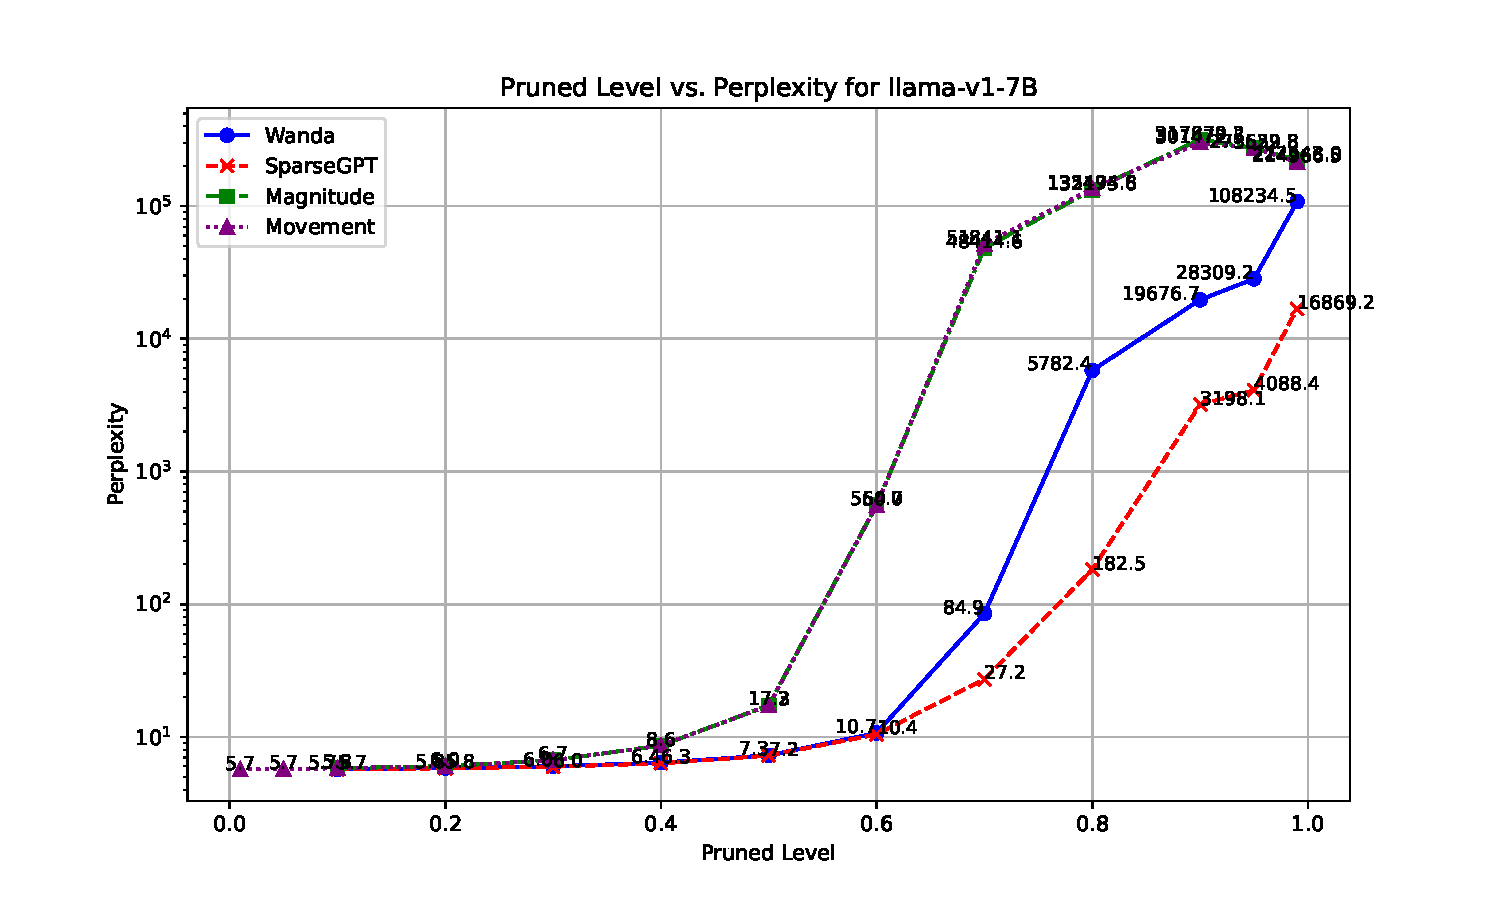
\includegraphics[width=0.8\linewidth]{fig1.pdf} 
\end{center}
\caption{Pruned Level vs. Perplexity for llama-v1-7B}
\label{fig:fig1} 
\end{figure}

\begin{figure}[h]
\begin{center}
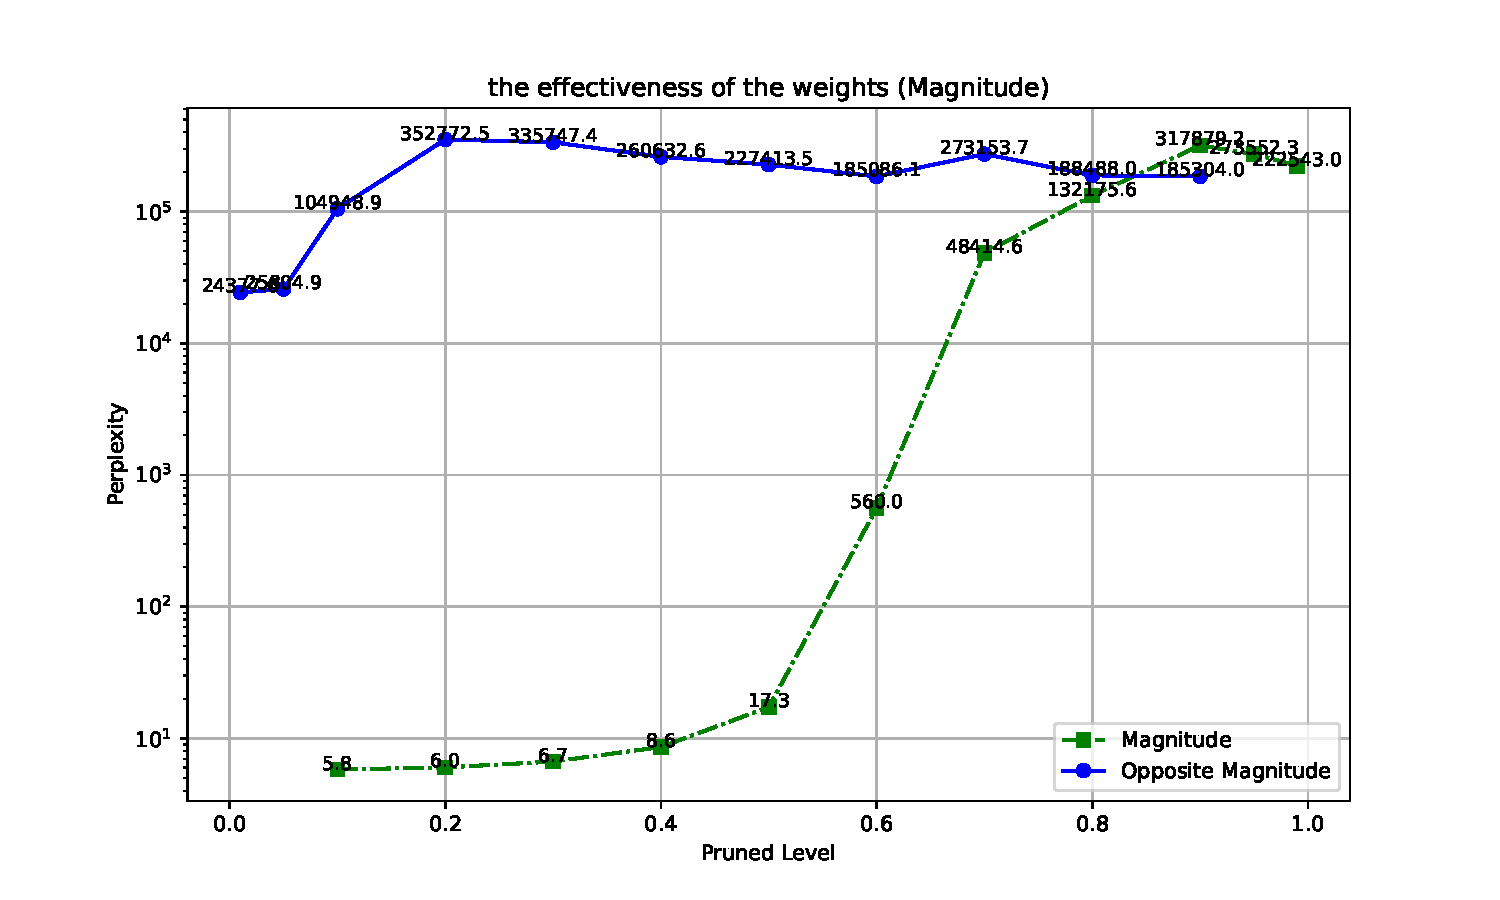
\includegraphics[width=0.8\linewidth]{fig2.pdf} 
\end{center}
\caption{Effectiveness of the weights indicator}
\label{fig:fig2} 
\end{figure}

\begin{figure}[h]
\begin{center}
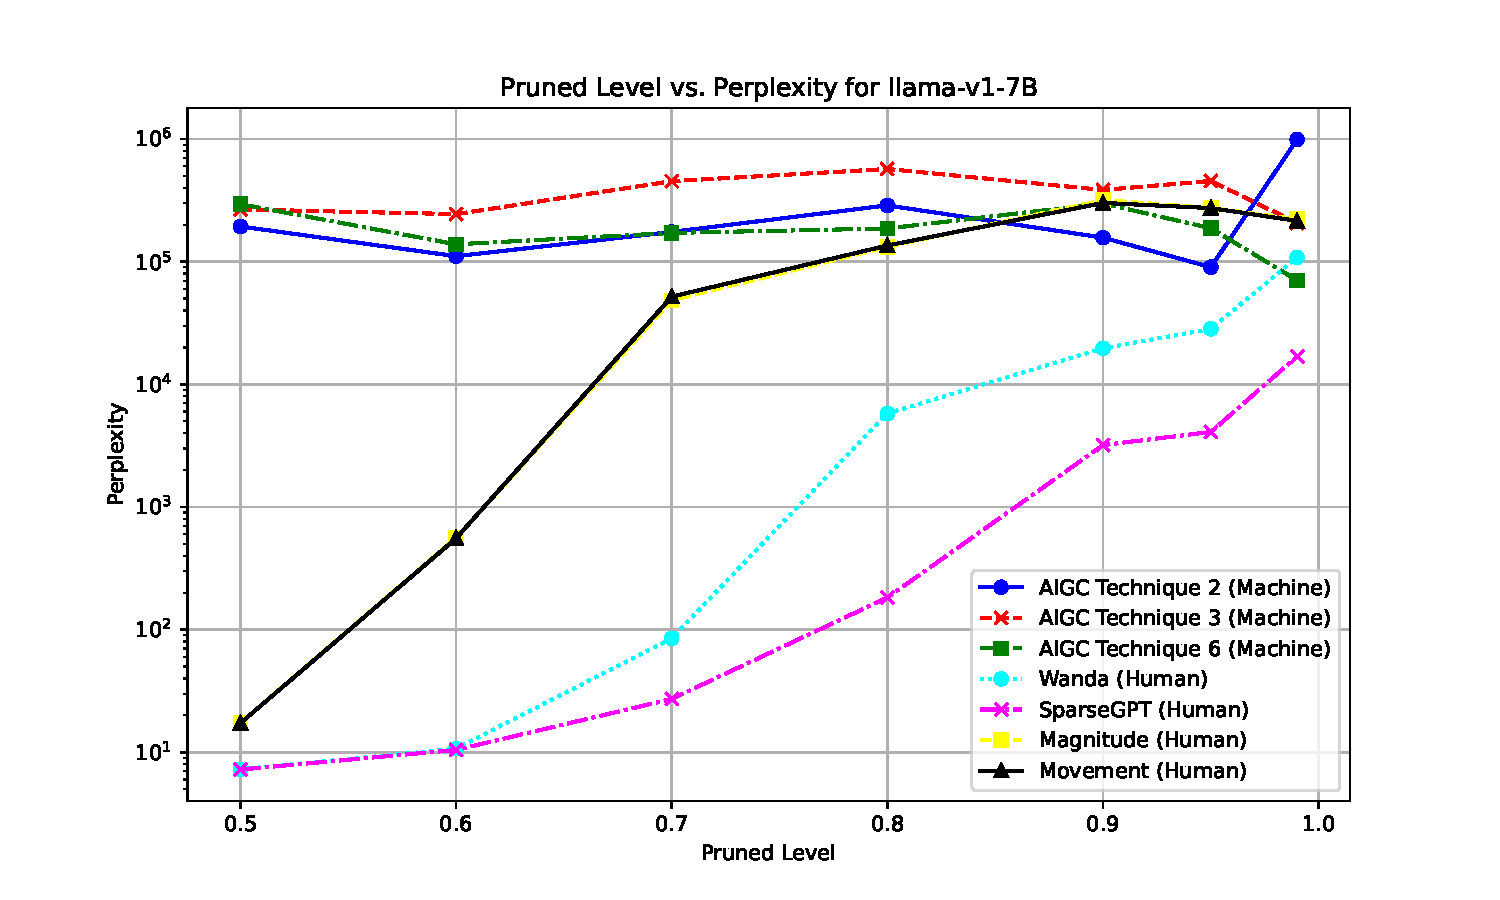
\includegraphics[width=0.8\linewidth]{fig3.pdf} 
\end{center}
\caption{Performance Evaluation between Machine \& Human}
\label{fig:fig3} 
\end{figure}

\subsubsection*{Author Contributions}
If you'd like to, you may include  a section for author contributions as is done
in many journals. This is optional and at the discretion of the authors.

\subsubsection*{Acknowledgments}
Use unnumbered third level headings for the acknowledgments. All
acknowledgments, including those to funding agencies, go at the end of the paper.

\bibliography{iclr2025_conference}
\bibliographystyle{iclr2025_conference}

\appendix
\section{Appendix}
You may include other additional sections here.


\end{document}